\begin{enumerate}
\item \begin{enumerate}
  \item D'après les définitions, l'angle orienté entre les vecteurs $\overrightarrow{i}$ et $\overrightarrow{\tau}(\theta)$ est 
\begin{displaymath}
 \widehat{(\overrightarrow{i} , \overrightarrow{\tau}(\theta))} = \theta + V(\theta)
\end{displaymath}
  \item Avec la remarque de l'énoncé relative aux bissectrices, il est immédiat que
\begin{displaymath}
 \widehat{(\Delta_\theta,\mathcal{R}_\theta)} = \theta + 2V(\theta) \mod \pi
\end{displaymath}
\end{enumerate}
\item Dans cette question le support de $M(\theta)$ est une cardioïde (courbe classique).
\begin{figure}
   \centering
   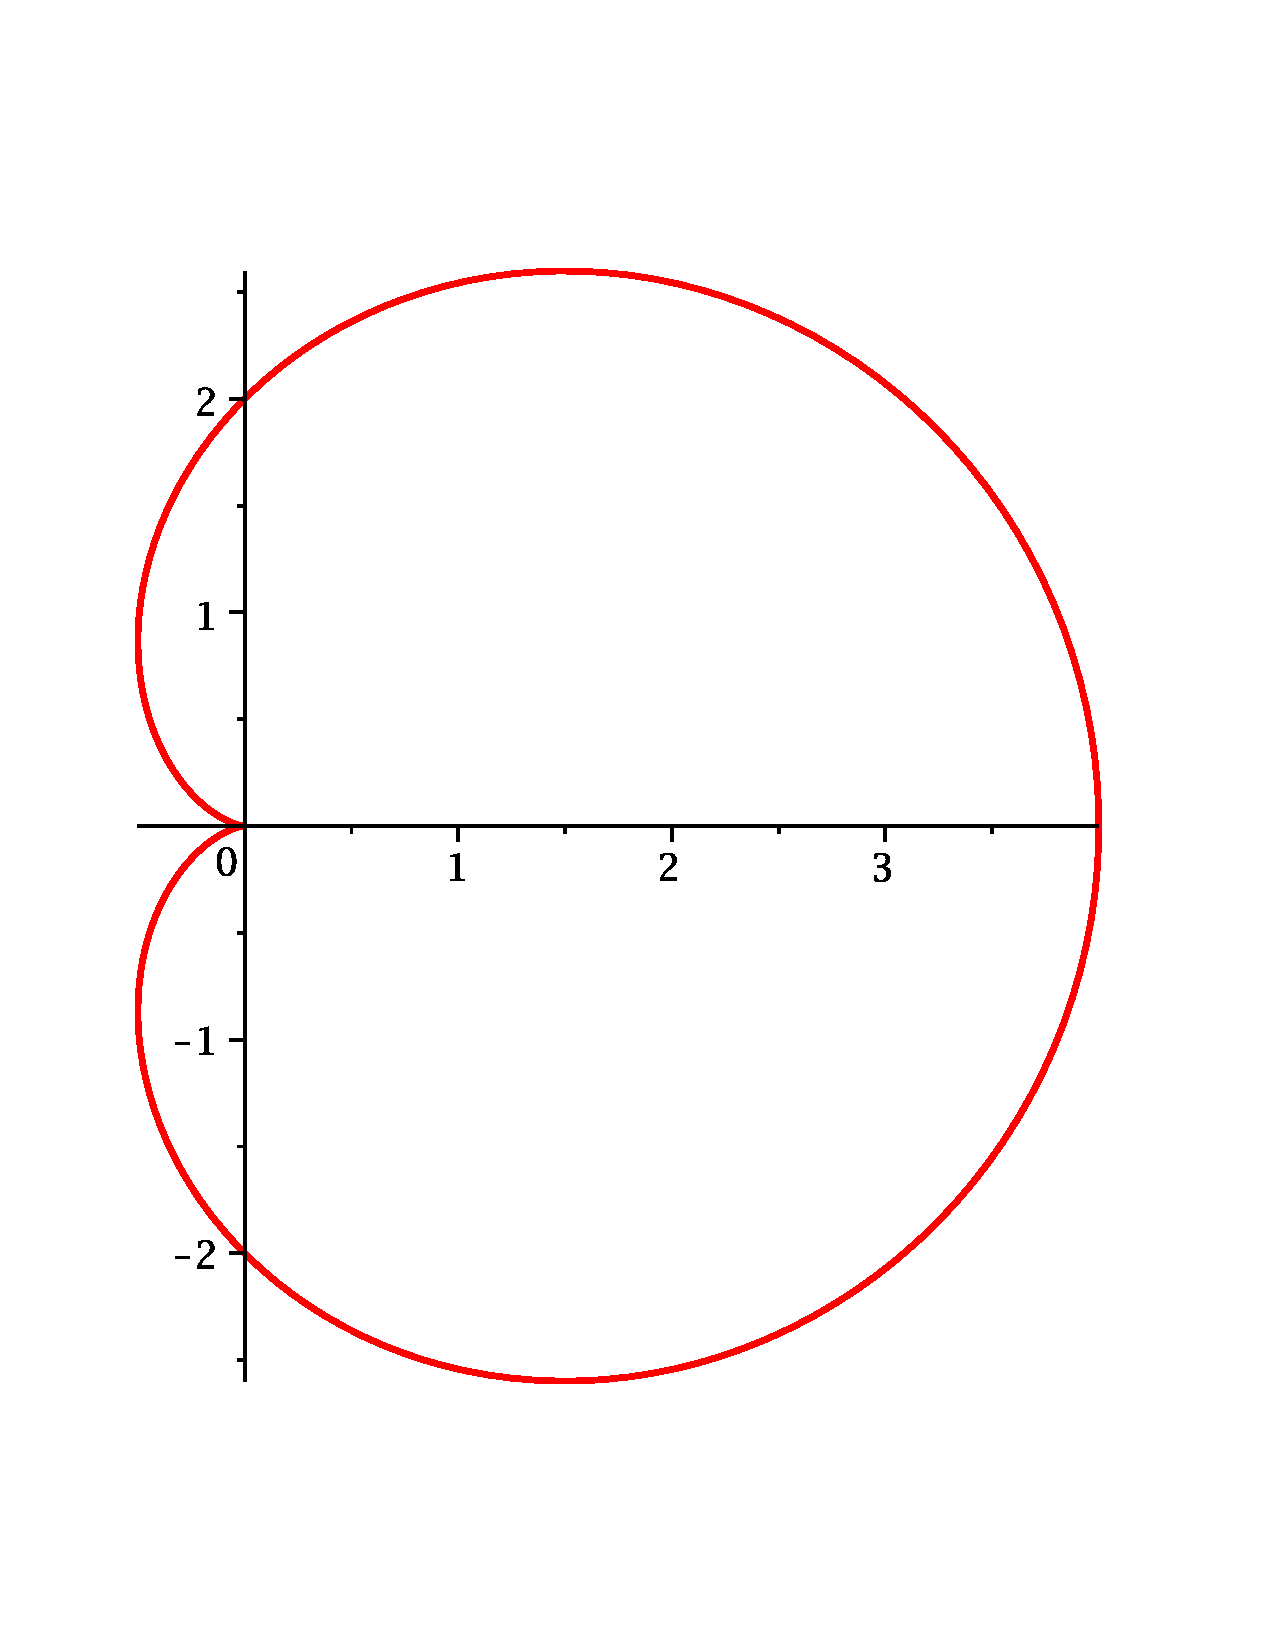
\includegraphics[scale=0.25]{Ccaustic_1.pdf}
   \caption{Question 2. Cardioïde pour $a=2$}
   \label{fig:Ccaustic_1}
\end{figure}
En calculant la dérivée de $M$, on peut mettre en facteur $2a\cos \frac{\theta}{2}$.
\begin{multline*}
\overrightarrow{M'}(\theta)
= 2a\cos \frac{\theta}{2}\left(-\sin \frac{\theta}{2} \overrightarrow{e}_{\theta}+\cos \frac{\theta}{2}\overrightarrow{e}_{\theta +\frac{\pi}{2}} \right)\\
= 2a\cos \frac{\theta}{2}
\left(
\cos \frac{\theta}{2}\overrightarrow{e}_{\theta +\frac{\pi}{2}} +
\sin \frac{\theta}{2} \overrightarrow{e}_{\theta+\frac{\pi}{2}+\frac{\pi}{2}}
 \right)
= 2a\cos \frac{\theta}{2} \overrightarrow{e}_{\theta +\frac{\pi}{2}+\frac{\theta}{2}}
\end{multline*}
donc 
\begin{displaymath}
V(\theta) = \frac{\theta}{2}+\frac{\pi}{2} 
\end{displaymath}
et, pour l'angle orienté entre les droites :
\begin{displaymath}
 \widehat{(\Delta_\theta,\mathcal{R}_\theta)} = \theta + 2V(\theta) = 2\theta \mod \pi
\end{displaymath}

\item Le support de la courbe $M(\theta)$ est ici le cercle de centre le point $A$ de coordonnées $(a,0)$ et qui passe par l'origine (voir cours).
\begin{figure}
   \centering
   \input{Ccaustic_3.pdf_t}
   \caption{Cercle support pour $\rho(\theta)=2a\cos \theta$}
   \label{fig:Ccaustic_3}
\end{figure}
En effet, en multipliant par $\rho$, l'équation devient 
\begin{displaymath}
 \rho^2 = 2a\rho \cos \theta 
\Leftrightarrow
x^2+y^2 = 2ax
\Leftrightarrow
(x-a)^2+y^2=a^2
\end{displaymath}
\begin{enumerate}
  \item Le calcul de la dérivée est analogue à celui de la question précédente, on obtient :
\begin{multline*}
 \overrightarrow{M'}(\theta) = 2a\overrightarrow{e_{2\theta + \frac{\pi}{2}}}
\Rightarrow
V(\theta)=\theta+\frac{\pi}{2}\\
\Rightarrow
\widehat{(\Delta_\theta,\mathcal{R}_\theta)} = \theta + 2V(\theta) = 3\theta \mod \pi
\end{multline*}
  \item On connait les coordonnées du point $M(\theta)$ de $\mathcal{R}_{\theta}$ et d'un vecteur directeur, on en déduit l'équation en utilisant le déterminant
\begin{multline*}
 \begin{vmatrix}
  x - 2a\cos^2\theta & \cos(3\theta)\\
  y -2a\cos(\theta)\sin(\theta) & \sin(3\theta)
 \end{vmatrix}=
 \begin{vmatrix}
  x - a(1+\cos(2\theta) & \cos(3\theta)\\
  y -a\sin(2\theta) & \sin(3\theta)
 \end{vmatrix}\\
=(x-a)\sin(3\theta)-y\cos(3\theta)
-a\left( \cos(2\theta)\sin(3\theta)-\sin(2\theta)\cos(3\theta)\right) \\
= (x-a)\sin(3\theta)-y\cos(3\theta) -a\sin(\theta)
\end{multline*}
On obtient donc l'équation de $\mathcal{R}_\theta$
\begin{displaymath}
(x-a)\sin(3\theta) -y\cos(3\theta)  - a\sin(\theta=0) \quad (\mathcal{R}_{\theta}) 
\end{displaymath}
Si on pose $t=3\theta - \frac{3\pi}{2}$, l'équation devient
\begin{displaymath}
(x-a)\cos(t)  +  y\sin(t) + a\cos(\frac{t}{3})=0 \quad (\mathcal R _\theta) 
\end{displaymath}
\end{enumerate}

\item D'après le cours, les formules de linéarisation sont :
\begin{align*}
 \cos(u) \cos(v) &=\frac{1}{2}\left( \cos(u+v) + \cos(u-v)\right) \\ 
 \sin(u) \sin(v) &=\frac{1}{2}\left( \cos(u-v) - \cos(u+v)\right) \\
 \cos(u) \sin(v) &=\frac{1}{2}\left( \sin(u+v) - \sin(u-v)\right)
\end{align*}


\item \begin{enumerate}
  \item On forme le système linéaire attaché à l'intersection des deux droites. Son déterminant vaut 1. On en déduit que les droites se coupent.\newline
  Notons $x(t)$ et $y(t)$ les coordonnées de $H(t)$. On ne cherche pas pour le moment à calculer ces coordonnées.\newline
  Elles vérifient l'équation de $\mathcal{R}_t$ c'est à dire
  \[(x(t)-a)\cos(t)  + y(t)\sin(t) +a\cos(\frac{t}{3})=0\]
  Dérivons cette fonction (elle est constante). On obtient
\begin{displaymath}
0=x'(t)\cos(t) + y'(t)\sin(t) 
\underset{=0}{\underbrace{- (x(t)-a)\sin(t)  + y(t)\cos(t) -\frac{a}{3}\sin(\frac{t}{3})}} 
\end{displaymath}
Comme les coordonnées de $H$ vérifient aussi la deuxième équation, on a encore 
\begin{displaymath}
x'(t)\cos t+y'(t)\cos t=0 
\end{displaymath}
donc $\overrightarrow{H'}(t)$ est orthogonal à 
\begin{displaymath}
\overrightarrow{e}_t=\overrightarrow{e}_{3\theta -\frac{3\pi}{2}} 
\end{displaymath}
Ce dernier vecteur est orthogonal à $\mathcal{R}_\theta$ donc $\mathcal{R}_\theta$ est tangent à la courbe des $H(t)$.
\begin{figure}
   \centering
   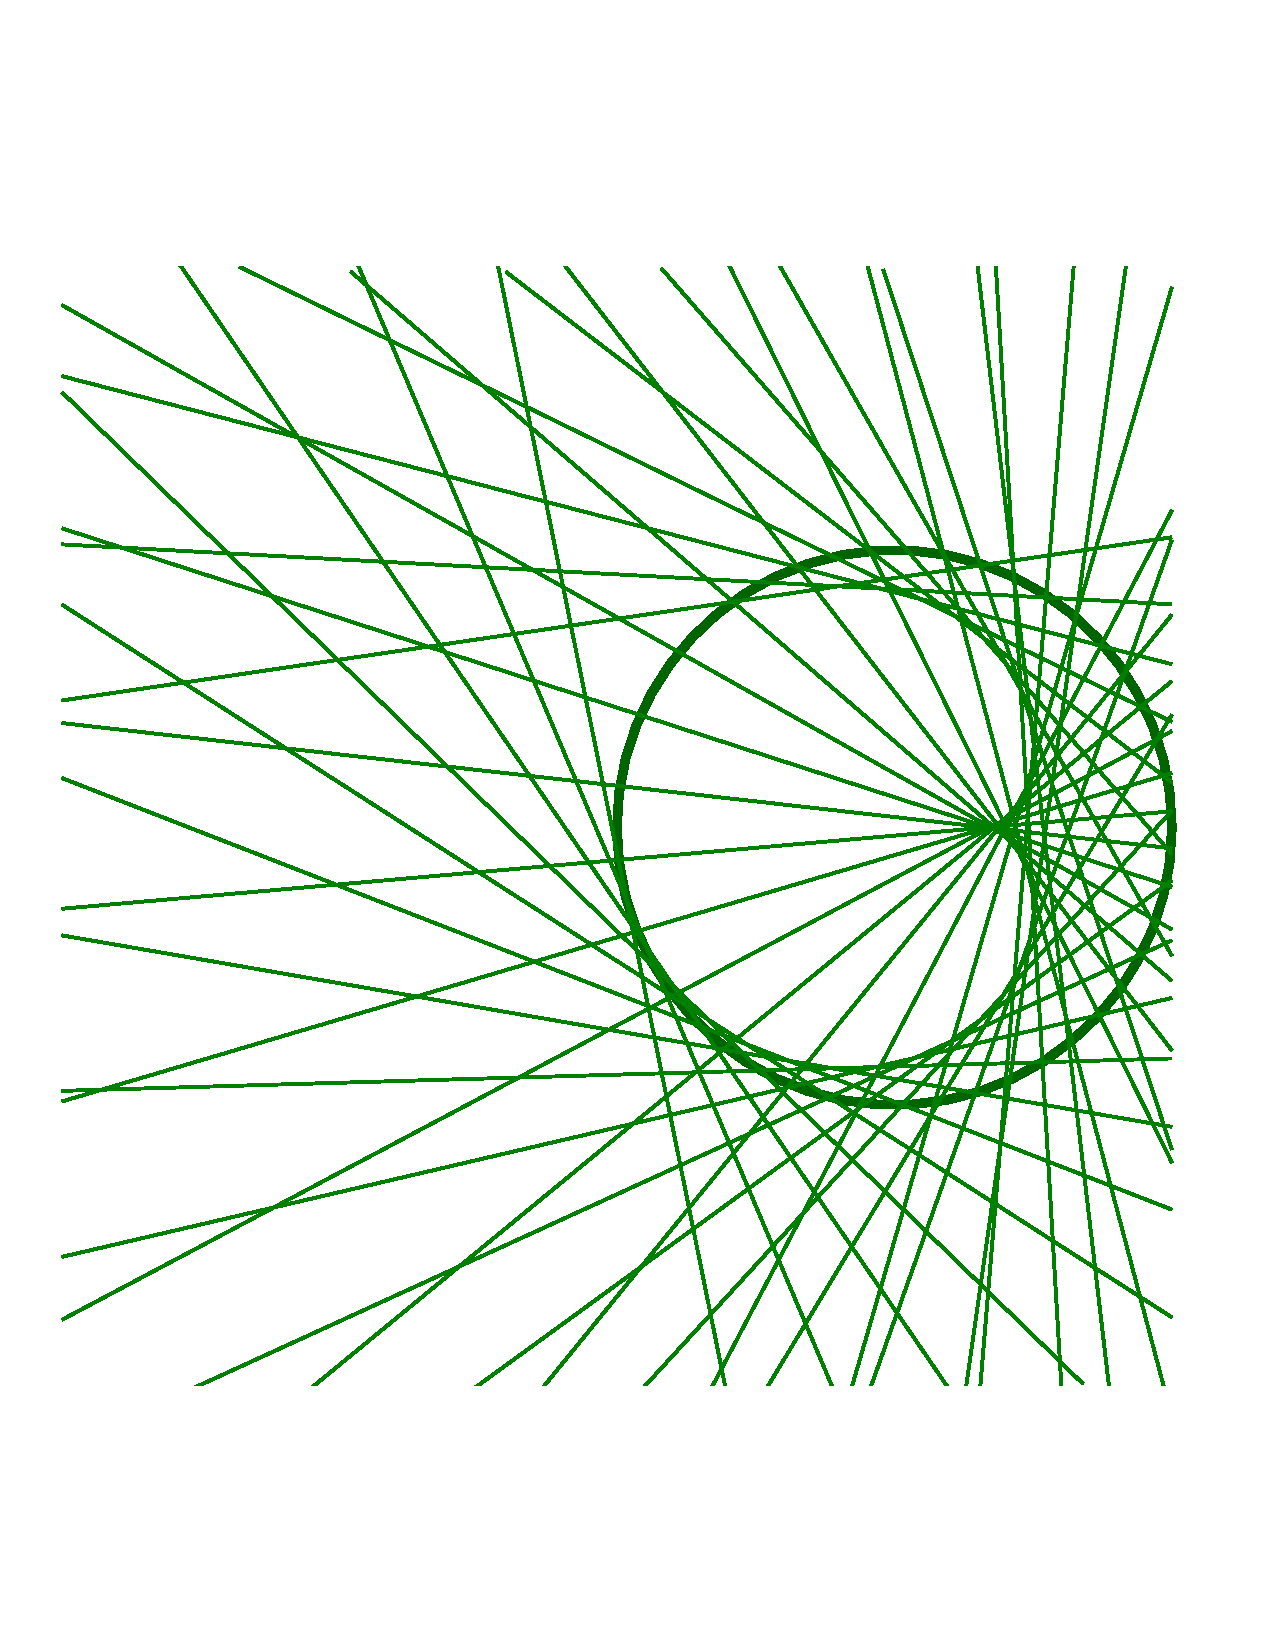
\includegraphics[scale=0.5]{Ccaustic_2.pdf}
   \caption{Tracé de 40 droites $\mathcal{R}_t$}
   \label{fig:Ccaustic_2}
\end{figure}

\item En résolvant par les formules de Cramer le système définissant $H(t)$, on obtient :
\begin{eqnarray*}
x(t)-a &=& -a \cos \frac{t}{3} \cos t -\frac{a}{3}\sin \frac{t}{3}\sin t \\
y(t) &=& \frac{a}{3} \cos t \sin \frac{t}{3}  -a\sin t \cos \frac{t}{3}
\end{eqnarray*}
On utilise ensuite les formules trigonométriques transformant les produits en sommes (linéarisation) pour obtenir
\begin{eqnarray*}
x(t) &= a &- \frac{a}{3}\cos \frac{4t}{3} -\frac{2a}{3}\cos \frac{2t}{3} \\
y(t) &=   &-\frac{a}{3} \sin \frac{4t}{3}  -\frac{2a}{3}\sin \frac{2t}{3}
\end{eqnarray*}
Ce qui donne, avec les notations de l'énoncé :
\[\alpha=-\frac{a}{3} , \beta = -\frac{2a}{3}\]
ou encore
\begin{displaymath}
 H(t) = A -\frac{a}{3}\,\overrightarrow{e_{\frac{4t}{3}}} - \frac{2a}{3}\,\overrightarrow{e_{\frac{2t}{3}}} 
\end{displaymath}

\item D'après les questions précédentes, calculer $\overrightarrow{H'(t)}$:
\begin{displaymath}
\overrightarrow{H'(t)}
=-\frac{4a}{9}
\left( 
  \overrightarrow{e_{\frac{4t}{3}+\frac{\pi}{2}}} + \overrightarrow{e_{\frac{2t}{3}+\frac{\pi}{2}}}
\right) 
=\frac{8a}{9}\cos \frac{t}{3}\overrightarrow{e}_{t-\frac{\pi}{2}} 
\end{displaymath}
Comme $\frac{t}{3}\in ]0,\pi[$, il existe un unique point stationnaire $\Omega$ qui est atteint pour $\frac{t}{3}=\frac{\pi}{2}$ d'où $\frac{2t}{3}=\pi$. Finalement:
\begin{multline*}
\Omega = H(\frac{3\pi}{2}) 
= A -\frac{a}{3}\overrightarrow i + \frac{2a}{3}\overrightarrow i 
= A + \frac{a}{3}\overrightarrow i \\
\text{ de coordonnées } (\frac{4a}{3},0) 
\end{multline*}

\item On calcule $\overrightarrow{\Omega H(t)}$ dans la base $(\overrightarrow{i},\overrightarrow{j})$ en utilisant systématiquement $\frac{2t}{3}$. On peut factoriser $1+\cos \frac{2t}{3}$ d'où
\[\overrightarrow{\Omega H(t)}=-\frac{2a}{3}(1+\cos \frac{2t}{3})\overrightarrow{e_{\frac{2t}{3}}}\]
On peut donc choisir
\[r(\varphi)=-\frac{2a}{3}(1+\cos \varphi)\]
La caustique par reflexion d'un cercle est symétrique par rapport à $Oy$ d'une courbe du type de la question 2. (cardioïde).
\end{enumerate}
\end{enumerate}
